\documentclass{article}
\usepackage{tikz}
\usepackage{amsmath}
\usepackage{amsfonts}
\usepackage{amssymb}

\begin{document}

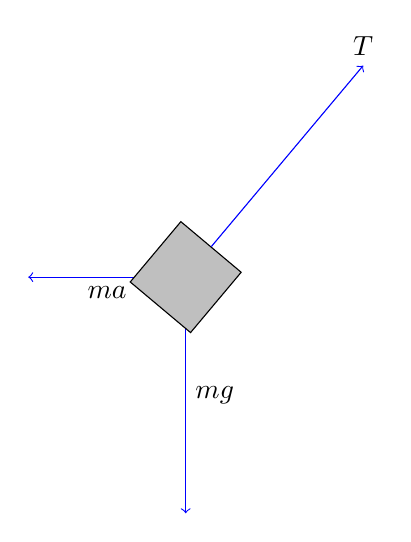
\begin{tikzpicture}[
    force/.style={draw=blue,fill=blue},
    m/.style={rectangle,draw=black,fill=lightgray,minimum size=1cm,thin},
    ]
    \draw[force,->] (0,0) -- (0,-3) node[midway, right] {$mg$};
    \draw[force,->] (0,0) -- (-2,0) node[midway, below] {$ma$};
    \begin{scope}[rotate=50]
    \node[m,transform shape] (M) {};
    \draw[force,->] (M.east) -- ++(3,0) node[above] {$T$};
    \end{scope}
\end{tikzpicture}

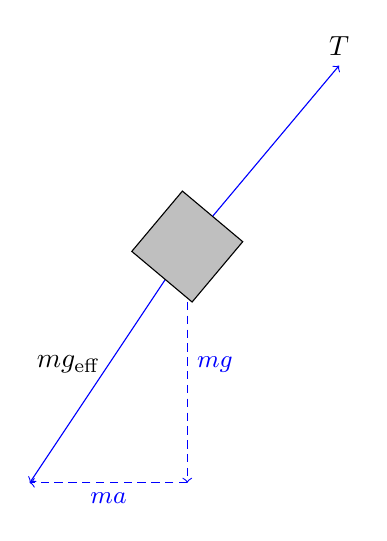
\begin{tikzpicture}[
    force/.style={draw=blue, fill=blue},
    component/.style={densely dashed, blue,font=\small},
    m/.style={rectangle,draw=black,fill=lightgray,minimum size=1cm,thin},
    ]
    \draw[component,->] (0,0) -- (0,-3) node[midway, right] {$mg$};
    \draw[component,->] (0,-3) -- (-2,-3) node[midway, below] {$ma$};
    \draw[force,->] (0,0) -- (-2,-3) node[midway, left] {$mg_\text{eff}$}; 
    \begin{scope}[rotate=50]
    \node[m,transform shape] (M) {};
    \draw[force,->] (M.east) -- (3,0) node[above] {$T$};
    \end{scope}
\end{tikzpicture}

\end{document}